\documentclass[conference]{IEEEtran}

\usepackage{cite}
\usepackage{url}
\usepackage{booktabs}
\usepackage{amsmath}
\usepackage{array}
\usepackage{tikz}
\usetikzlibrary{arrows.meta,positioning}

\newcommand{\paperauthorname}{Shangjae Lee}
\newcommand{\paperaffiliation}{Kyungpook National University}
\newcommand{\paperemail}{dltkdwo31@knu.ac.kr}

\title{Anchor-Constrained Feature-Similarity Ensembling for Multimodal Lifelog State Prediction}

\author{
\IEEEauthorblockN{\paperauthorname}
\IEEEauthorblockA{\paperaffiliation\\
\paperemail}
}

\begin{document}
\maketitle

\begin{abstract}
Predicting daily sleep and stress states from lifelogs is difficult when labels are scarce, observations are participant-dependent, and validation does not match the hidden test distribution. We present an anchor-constrained ensemble for seven binary targets in the 5th ETRI Human Understanding AI Paper Challenge. A stable sequence-based probability model is augmented with a same-participant nearest-neighbor signal computed from four sensor feature families. Target-specific similarity predictions are first blended conservatively into a secondary model, then shrunk halfway toward the stable public anchor. On 450 labeled person-days from 10 participants, the resulting model obtains a local mean log loss of 0.534000 and a DACON public score of 0.5960832519, improving the previous anchor by 0.0053280490. More aggressive models achieved much lower local loss but transferred poorly. Ablations and three later public probes show that small local gains are not sufficient evidence near the anchor. The main result is therefore a practical validation and risk-control procedure for multimodal lifelog prediction under small-sample distribution shift.
\end{abstract}

\begin{IEEEkeywords}
lifelog, multimodal sensing, sleep prediction, stress prediction, nearest neighbors, ensemble learning
\end{IEEEkeywords}

\section{Introduction}
Continuous sensing from smartphones and wearables provides a nonintrusive view of activity, physiology, mobility, and device use. The ETRI lifelog datasets combine these streams with subjective reports and sleep-health outcomes, enabling models of daily human state \cite{oh2025etri,oh2024challenge}. Their small number of participants and heterogeneous routines, however, make generalization unusually fragile: a pattern may represent a participant's stable habit rather than a transferable state marker.

The 5th ETRI Human Understanding AI Paper Challenge asks participants to predict seven daily binary targets from multimodal lifelog data \cite{dacon2026rules}. Our experiments exposed a second difficulty beyond ordinary overfitting. A candidate with local mean log loss 0.378934 obtained a much worse public score of 0.6698787318, whereas several models around local 0.54 transferred near public 0.60. Consequently, selecting the local minimum was actively misleading.

We address this setting with an anchor-constrained probability ensemble. The model combines a stable sequence-based prediction with a low-weight, same-participant feature-similarity estimate. The final prediction is shrunk toward a previously public-scored anchor, limiting the effect of a locally selected component. Our contributions are: (1) a target-specific similarity formulation over domain-aligned sensor families; (2) an anchor-shrink strategy that improved the public score while bounding prediction movement; and (3) an empirical promotion protocol that separates stable near-anchor comparisons from failed local frontiers. We also report negative results because they delimit what the public improvement does and does not establish.

\begin{figure*}[t]
\centering
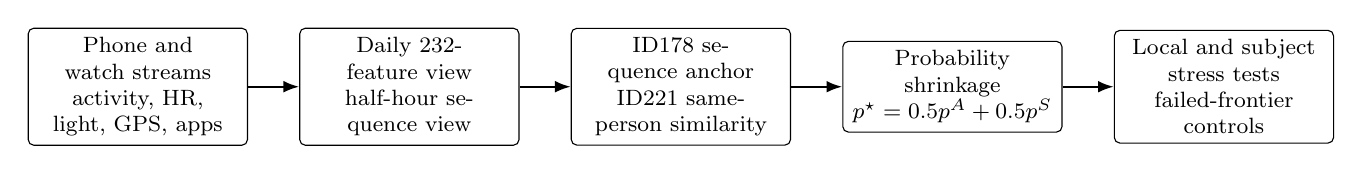
\begin{tikzpicture}[
  node distance=0.65cm,
  box/.style={draw, rounded corners=2pt, align=center, minimum height=1.05cm, text width=2.55cm, font=\footnotesize},
  arrow/.style={-{Latex[length=2mm]}, thick}
]
\node[box] (sensors) {Phone and watch streams\\activity, HR, light, GPS, apps};
\node[box, right=of sensors] (repr) {Daily 232-feature view\\half-hour sequence view};
\node[box, right=of repr] (sources) {ID178 sequence anchor\\ID221 same-person similarity};
\node[box, right=of sources] (shrink) {Probability shrinkage\\$p^\star=0.5p^A+0.5p^S$};
\node[box, right=of shrink] (gates) {Local and subject stress tests\\failed-frontier controls};
\draw[arrow] (sensors) -- (repr);
\draw[arrow] (repr) -- (sources);
\draw[arrow] (sources) -- (shrink);
\draw[arrow] (shrink) -- (gates);
\end{tikzpicture}
\caption{Overview of the anchor-constrained modeling and promotion workflow. Labels are used only inside the model-training or same-participant neighbor sets; leaderboard feedback enters the final risk audit, not model fitting.}
\label{fig:workflow}
\end{figure*}

\section{Data and Evaluation}
\subsection{Task and Features}
The data contain 450 labeled and 250 test person-days from 10 participants. Training dates span June 4 to November 15, 2024; test dates span July 7 to November 20, 2024. Test days are interleaved with labeled days for each participant rather than forming a pure future holdout. The processed representation has 232 features: screen (17), phone activity (27), pedometer (27), heart rate (39), light (36), place and mobility (28), app usage (27), and demographic/calendar features (12). Raw sources include phone charge, activity, ambience, Bluetooth, GPS, light, screen and app events, Wi-Fi, and watch heart rate, light, and steps.

Participant contributions are unequal: labeled days range from 33 to 57 and test days from 19 to 32 per participant. Positive-label prevalence ranges from 0.496 for Q1 to 0.682 for S1. This is large enough to make an unstratified random split sensitive to individual baselines. The hidden test geometry is also heterogeneous. Six participants have two contiguous test blocks, while four have five to seven fragmented blocks. We therefore preserve participant identity during validation and treat a purely chronological split only as a stress test.

The subjective targets are sleep quality (Q1), low physical fatigue before sleep (Q2), and low stress before sleep (Q3). The objective sleep targets represent guideline adherence for total sleep time (S1), sleep efficiency (S2), sleep onset latency (S3), and wake after sleep onset (S4). Following the competition metric, we use mean binary log loss over the seven targets:
\begin{equation}
\mathcal{L}=-\frac{1}{7N}\sum_{i=1}^{N}\sum_{t=1}^{7}
\left[y_{it}\log p_{it}+(1-y_{it})\log(1-p_{it})\right].
\end{equation}

Prior work has represented synchronized lifelog channels as images \cite{na2025pixleep} and learned cross-modal time-series representations with latent masking \cite{deldari2024crossl}. Our limited sample size instead favored strong shrinkage and compact probability overlays. We retained raw sequence information through ROCKET-style random convolution features \cite{dempster2020rocket}, but used sensor-family nearest neighbors for the final correction.

\subsection{Validation Lenses}
The primary local lens is five-fold, within-participant blocked validation designed to resemble the interleaved test pattern. We additionally evaluated subject-hole, leave-one-subject-out (LOSO), temporal, and test-boundary stress lenses. The public leaderboard is used only as sparse post-hoc evidence from submitted candidates; it is not treated as a validation fold.

Primary validation folds contain 85--95 days and preserve observations from all participants where possible. Subject-hole folds remove contiguous windows within each participant; LOSO evaluates transfer to an unseen participant; and boundary holdouts emphasize labeled days adjacent to the known test blocks. These lenses answer different questions and are not averaged into a synthetic score. The primary lens ranks candidates, while the others can veto a candidate whose apparent gain depends on one split geometry.

Feature-similarity hyperparameters were selected on the full primary out-of-fold diagnostic, not by nested cross-validation. Thus, the reported 0.534000 is a model-selection score and is optimistically biased. We explicitly preserve this limitation and use the official public score as the final comparative result. Label-free median imputation and standardization used the combined train/test covariate matrix; all neighbor outcomes for validation and test queries came only from labeled training rows.

\section{Method}
\subsection{Stable Sequence Anchor}
The public anchor, denoted $p^{A}$ (experiment ID178), is a target-wise ensemble built on processed daily features and half-hour sequence summaries. Deterministic random convolution features are followed by regularized logistic heads. Depending on the target, 192 or 384 kernels are used and the sequence probability receives weight 0.11--0.165; S3 retains its preceding base prediction. Although the raw sequence heads alone overfit, their small probability overlays produced a stable public score of 0.6014113009. We use this scored model as an empirical anchor rather than claiming that its local score is unbiased.

\subsection{Same-Participant Feature Similarity}
We partition the processed variables into four families: date/time (29 features), screen/app (53), movement/GPS (44), and light/heart rate (114). Missing values are median-imputed and each feature is standardized. For a query day $i$ and a labeled day $j$ belonging to the same participant, family-specific distance is
\begin{equation}
d_{ij}^{(f)}=\sqrt{\frac{1}{|f|}\lVert z_i^{(f)}-z_j^{(f)}\rVert_2^2}
+\lambda\log(1+|\tau_i-\tau_j|),
\end{equation}
where $z^{(f)}$ is the standardized feature vector and $\tau$ is calendar date. The similarity estimate $s_{it}$ is the mean label among the $k$ nearest eligible days of the same participant, with $k\in\{1,3,7\}$ and $\lambda\in\{0,0.03,0.1\}$. This follows the local-neighborhood intuition of nearest-neighbor classification \cite{cover1967nearest} while preventing labels from other participants from defining an individual's baseline.

For each target, a small blend with a preceding model $p^{B}$ forms the similarity source:
\begin{equation}
\begin{aligned}
p^{S}_{it}&=(1-w_t)p^{B}_{it}+w_t s_{it},\\
w_t&\in\{0.005,0.01,0.02,0.03,0.05,0.07\}.
\end{aligned}
\end{equation}
Table~\ref{tab:configs} lists the selected target-specific configurations. The search remained deliberately narrow, and all overlay weights were at most 0.07.

\begin{table}[t]
\centering
\caption{Selected feature-similarity configurations.}
\label{tab:configs}
\begin{tabular}{@{}llllr@{}}
\toprule
Target & Family & $k$ & $\lambda$ & $w_t$ \\
\midrule
Q1 & screen/app & 1 & 0 & 0.07 \\
Q2 & date/time & 1 & 0.10 & 0.03 \\
Q3 & date/time & 1 & 0 & 0.03 \\
S1 & date/time & 1 & 0.03 & 0.02 \\
S2 & move/GPS & 7 & 0.03 & 0.07 \\
S3 & screen/app & 1 & 0.03 & 0.05 \\
S4 & light/HR & 3 & 0.03 & 0.07 \\
\bottomrule
\end{tabular}
\end{table}

\subsection{Anchor-Constrained Shrinkage and Promotion}
The final model (ID342) is the midpoint between the stable public anchor and the similarity source:
\begin{equation}
p^{\star}_{it}=(1-\alpha)p^{A}_{it}+\alpha p^{S}_{it},\qquad \alpha=0.50.
\end{equation}
This second shrinkage reduced the maximum test-probability movement relative to $p^A$ from the unshrunk source while retaining half of its locally useful direction. The resulting mean and maximum absolute test changes were 0.01846 and 0.09391.

Candidate promotion used three checks. First, target and mean losses had to improve under the primary lens and remain plausible under subject-hole and LOSO stress tests. Second, probability movement was compared with two known failed directions: ID287, an extreme local frontier, and ID329, a guarded candidate that still failed to improve the public anchor. Third, every scored result was tied to a prediction artifact, experiment record, submission file, and official score. Failed-frontier rows were not deleted; they served as controls for later candidate geometry.

For candidate $c$ and anchor $A$, we recorded mean and maximum test movement, $m_1=\frac{1}{7N}\sum_{it}|p^c_{it}-p^A_{it}|$ and $m_\infty=\max_{it}|p^c_{it}-p^A_{it}|$. These quantities do not estimate accuracy; they bound how much an unscored model can invalidate what is known about the anchor. We also measured cosine projection onto the ID287 and ID329 prediction differences. Promotion required small movement and no dominant alignment with either failed direction. The thresholds were operating safeguards fixed for the final slate, not tuned accuracy metrics.

\section{Results}
Table~\ref{tab:target_losses} shows that the similarity source improved all seven primary-lens target losses relative to the public anchor. The largest reductions occurred for Q1 and S4. Midpoint shrinkage necessarily gives up part of these local gains, but limits reliance on the non-nested source selection.

\begin{table}[t]
\centering
\caption{Primary-lens log loss by target (lower is better).}
\label{tab:target_losses}
\begin{tabular}{@{}lrrr@{}}
\toprule
Target & Anchor ID178 & Similarity ID221 & Final ID342 \\
\midrule
Q1 & 0.551916 & 0.544061 & 0.545848 \\
Q2 & 0.556679 & 0.550171 & 0.551609 \\
Q3 & 0.567090 & 0.562231 & 0.563226 \\
S1 & 0.471630 & 0.467117 & 0.466643 \\
S2 & 0.529556 & 0.528881 & 0.529101 \\
S3 & 0.490893 & 0.489489 & 0.489945 \\
S4 & 0.602700 & 0.588980 & 0.591629 \\
\midrule
Mean & 0.538638 & 0.532990 & 0.534000 \\
\bottomrule
\end{tabular}
\end{table}

Table~\ref{tab:public_results} reports the public-scored controls. ID342 improved ID178 by 0.0053280490 and the immediately preceding best score of 0.6006206286 by 0.0045373767. The recent slate also preserved local ordering: ID342 outperformed ID339 and ID338 both locally and publicly. In contrast, ID287 demonstrates that unrestricted local-frontier selection can reverse the ranking.

\begin{table}[t]
\centering
\caption{Public-scored models used as transfer controls.}
\label{tab:public_results}
\begin{tabular}{@{}lrrl@{}}
\toprule
ID & Local & Public & Role \\
\midrule
342 & 0.534000 & 0.596083252 & final anchor \\
339 & 0.536441 & 0.598518779 & sequence summary \\
338 & 0.537861 & 0.599214518 & random-conv edit \\
337 & 0.538066 & 0.600620629 & low-movement edit \\
340 & 0.538426 & 0.601379175 & Q2 sequence edit \\
329 & 0.516718 & 0.601790858 & guarded failure \\
287 & 0.378934 & 0.669878732 & frontier failure \\
178 & 0.538638 & 0.601411301 & prior anchor \\
\bottomrule
\end{tabular}
\end{table}

To quantify this effect, Table~\ref{tab:alignment} compares local/public rank agreement under progressively stricter control sets. Pairwise agreement is the fraction of candidate pairs ordered identically by local and public score. Removing only the extreme ID287 is insufficient because ID329 remains locally attractive but publicly weaker than ID178. After excluding both preidentified failed frontiers, the six remaining models have exact rank agreement. The same exact ordering holds for the three-candidate June 23 slate across all frozen local lenses. This analysis is diagnostic rather than a recipe for deleting inconvenient runs: the exclusions were defined by their prior public failures, and both rows remain visible as negative controls.

\begin{table}[t]
\centering
\caption{Full-OOF alignment with public ranking.}
\label{tab:alignment}
\begin{tabular}{@{}lrrr@{}}
\toprule
Candidate set & $n$ & Spearman & Pairwise \\
\midrule
All scored & 8 & $-0.167$ & 0.536 \\
Exclude ID287 & 7 & 0.250 & 0.714 \\
Exclude ID287/329 & 6 & 1.000 & 1.000 \\
June 23 slate & 3 & 1.000 & 1.000 \\
\bottomrule
\end{tabular}
\end{table}

Three final Q3 app-name lexicon anti-signal variants provide a prospective near-anchor check. Their public scores were 0.5963391483, 0.5963352712, and 0.5961947552: all worse than ID342 despite small local improvements. Other plausible additions---historical weather and air quality, sleep-boundary proxies, subject-state representations, and temporal convolution models---also failed the frozen local promotion gates and were not included.

The source-to-anchor comparison is also informative at target level. Relative to ID178, ID342 reduces primary-lens loss by 0.006068 on Q1, 0.005071 on Q2, 0.003864 on Q3, 0.004987 on S1, 0.000455 on S2, 0.000948 on S3, and 0.011071 on S4. Thus, Q1 and S4 account for much of the local gain, consistent with their screen/app and light/heart-rate families. The improvement is not confined to one target, but the tiny S2/S3 changes caution against claiming that all sensor families contributed equally.

\section{Negative Evidence and Reproducibility}
Table~\ref{tab:negative} summarizes representative post-anchor routes evaluated with the frozen gate. Weather and air quality were plausible contextual signals, but historical KMA ASOS features produced only an unstable S4 movement, and the AirKorea 2024 Daejeon archive yielded no promoted target. Sleep-boundary and temporal-convolution probes did not pass Q3/S3 stability checks. A broader registered-source scan evaluated 450 target/model configurations over circadian, GPS-topology, phone/watch-discordance, proximity, and app-semantic matrices; none passed the ID342 gate. These results are not evidence that the modalities are irrelevant. They show that their measured increments were too small or unstable under this sample and validation design.

\begin{table}[t]
\centering
\caption{Representative routes rejected after ID342.}
\label{tab:negative}
\begin{tabular}{@{}p{0.30\linewidth}p{0.18\linewidth}p{0.39\linewidth}@{}}
\toprule
Route & Focus & Gate evidence \\
\midrule
Q3 app lexicon & Q3 & three public scores worse \\
Sleep boundary & Q3/S3 & no stable target pass \\
Tiny temporal CNN & Q3/S3 & no stable target pass \\
KMA ASOS & S4 & small, unstable change \\
AirKorea 2024 & Q3/S4 & zero promoted targets \\
Registered sources & all & 0/450 configurations \\
Historical ETRI & Q2/Q3 & Q2 relation only \\
\bottomrule
\end{tabular}
\end{table}

Reproducibility was enforced at the artifact level. ID342 has a one-to-one mapping among its experiment record, out-of-fold matrix, test matrix, notebook snapshot, submission CSV, submission-log row, and DACON submission identifier 1467937. The stored CSV hash is \texttt{02f622e1e9c68257...e13b394}; the official submission time is June 23, 2026, 23:30:37 KST. The final predictions reconstruct exactly as the 0.5/0.5 blend of ID178 and ID221. This lineage check prevents an unsubmitted local row from being reported as the final model.

The package excludes raw lifelogs and credentials. It includes the IEEE source, bibliography, metadata extracted from the source, lineage manifest, and commands for regenerating the audit reports. Random-convolution seeds and kernel counts are retained in the experiment metadata. The feature-similarity source can be regenerated from the target-specific settings in Table~\ref{tab:configs}; however, because its selection is non-nested, reproducing the number 0.534000 should not be interpreted as independent validation.

\section{Discussion and Limitations}
The result supports a narrow conclusion: conservative, domain-grouped similarity can improve a stable multimodal anchor when the correction is small. It does not establish that feature similarity is universally superior to end-to-end temporal modeling. Only 10 participants are available, the primary hyperparameter search is not nested, and train/test covariates participate in label-free scaling. Moreover, the anchor and promotion policy were developed after observing a limited set of public scores, so the public result is comparative competition evidence rather than an untouched test-set estimate.

The failed controls nevertheless reveal a useful operational pattern. When the sample is small and participant routines dominate, a dramatic local gain may indicate validation exploitation. Public-anchor shrinkage acts as regularization in prediction space, while failed-frontier alignment turns previous mistakes into explicit controls. Future work should evaluate the procedure with fully nested participant-aware selection, bootstrap uncertainty across person-days, and a private holdout from new participants. Self-supervised multimodal pretraining may then provide a genuinely independent source rather than another local recombination.

\section{Conclusion}
We presented an anchor-constrained feature-similarity ensemble for seven sleep and stress targets. The final model reduced the DACON public log loss from 0.6014113009 to 0.5960832519 while keeping prediction movement small. More importantly, the study shows why local loss, participant-aware stress tests, prediction geometry, and negative public controls must be considered together in small-sample lifelog modeling.

\bibliographystyle{IEEEtran}
\bibliography{references}

\end{document}
